%\begin{figure}[htb]
%\centering
%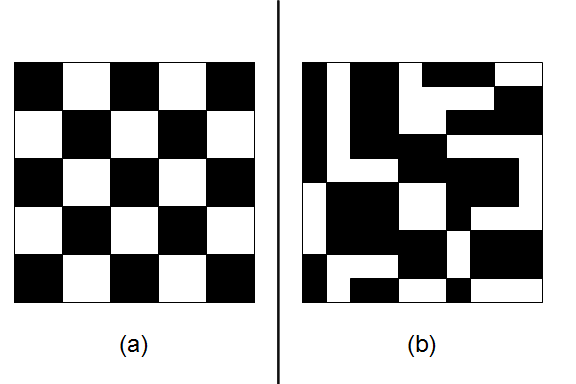
\includegraphics[width=\linewidth]{./graphics/checkers}
%\caption{Monte Carlo Checkerboard Example}
%\label{checker}
%\end{figure}

\begin{center}
\section{Conclusions}
\label{sec:Results}
\end{center}
\aboveSubSecSkip
% Summarize effects of results and express future work ideas



\subsection{Future Work}
There is still significant work that can be done to develop the discrete maximum principle and its applications in \gls{imc} radiative heat transfer codes.  In particular, the next logical implementation step is to build a routine whereby the user is given an appropriate time step for the problem and choice of spatial step when a violation is predicted.  Unfortunately, the limiting time step is dependent on the estimated energy deposited in the cell, which in turn is dependent on time step itself, so an iterative procedure would be necessary, although I expect a simple Euler method could be used to swiftly find such a time step for the most limiting cell in the problem.  

Additionally, work is ongoing with Dr. Wollaber at Los Alamos National Laboratory to determine necessary and sufficient conditions to bound the discrete maximum principle in a somewhat more robust way than has been done here.  As of this writing, a necessary condition has been determined using a purely absorbing (time step approaches zero and Fleck factor approaches unity) scheme; however, the sufficient purely scattering (time step approaches zero and Fleck factor approaches zero) is very difficult to analyze analytically \cite{TODO}.

Associated work is also ongoing to use partial Monte Carlo runs at each time step to increase the implicitness of the solution method.  In particular, work performed by Alex Long in association with Lawrence Livermore National Laboratory has shown the overheating event can be diminished using this increasingly implicit methodology.  It would be significant to investigate using this updated information to adjust the discrete maximum principle limit as well; however, since this update step decreases the severity of the limit, it is likely the run would be flagged as a likely violation before the update step, so some consideration would be necessary to determine the best way to implement this improved check.
\\ **TODO other future work? %%%%%%%%%%%%